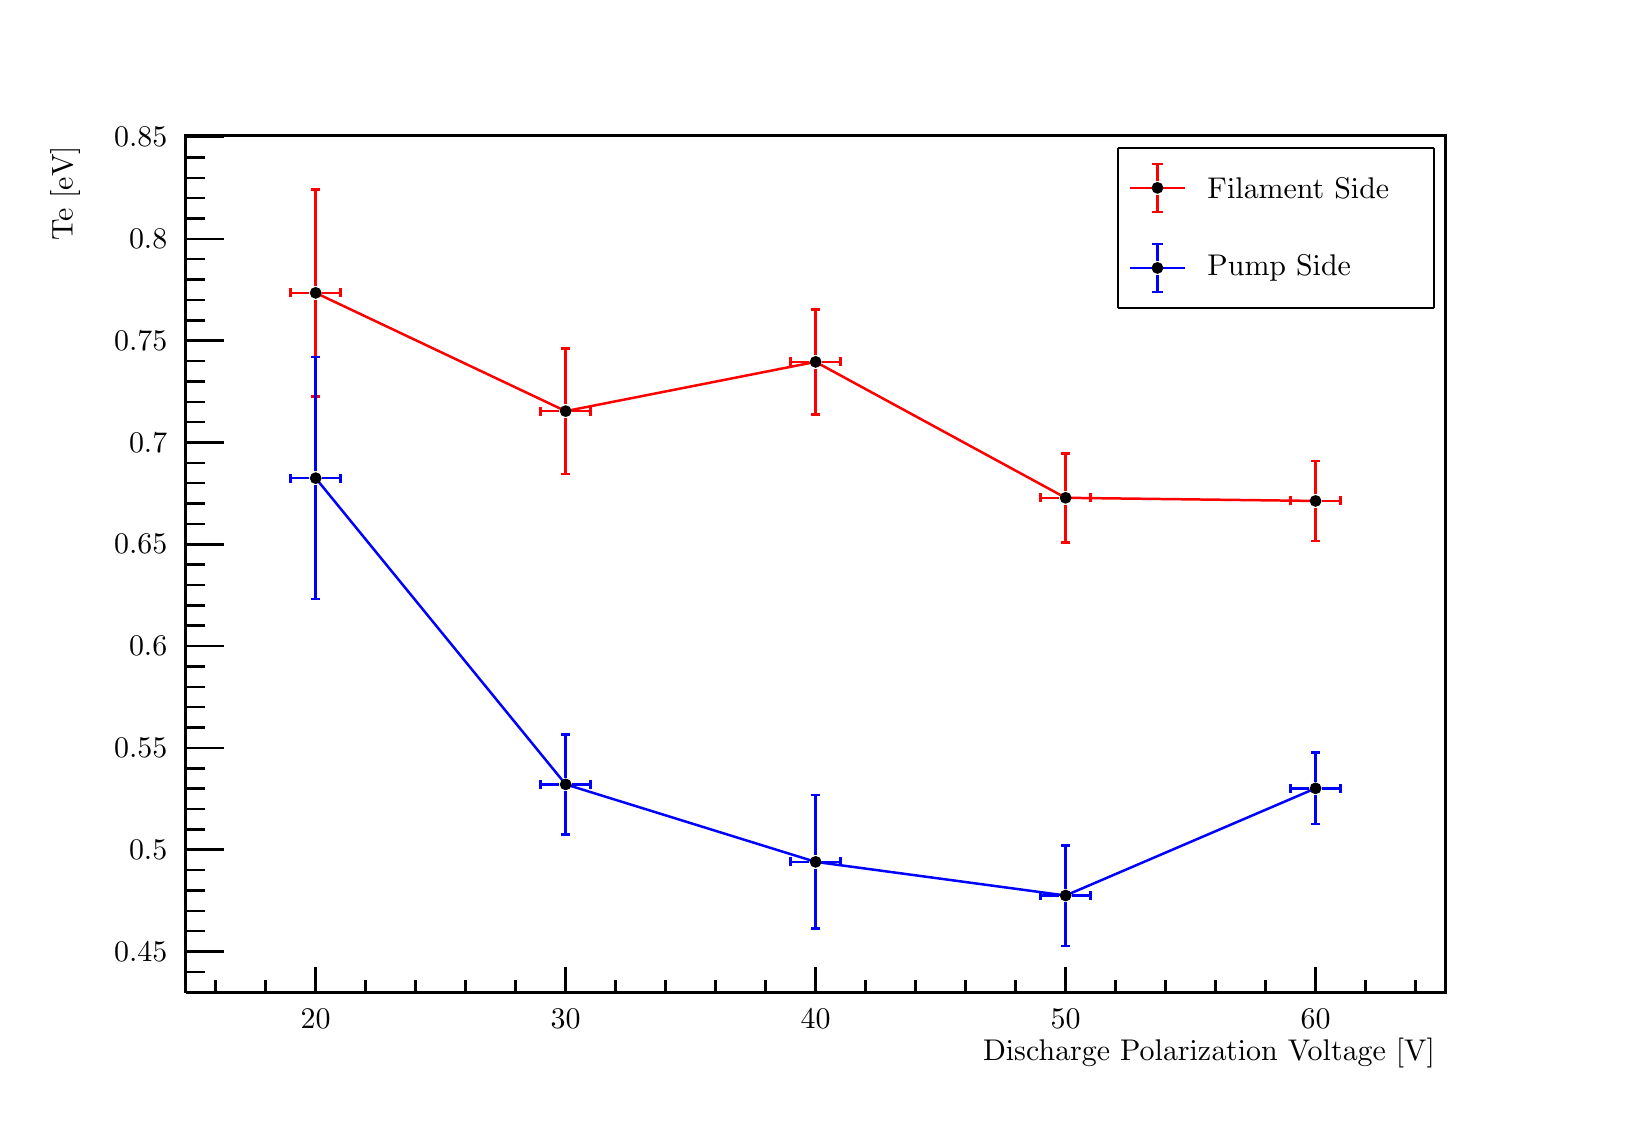
\begin{tikzpicture}
\pgfdeclareplotmark{cross} {
\pgfpathmoveto{\pgfpoint{-0.3\pgfplotmarksize}{\pgfplotmarksize}}
\pgfpathlineto{\pgfpoint{+0.3\pgfplotmarksize}{\pgfplotmarksize}}
\pgfpathlineto{\pgfpoint{+0.3\pgfplotmarksize}{0.3\pgfplotmarksize}}
\pgfpathlineto{\pgfpoint{+1\pgfplotmarksize}{0.3\pgfplotmarksize}}
\pgfpathlineto{\pgfpoint{+1\pgfplotmarksize}{-0.3\pgfplotmarksize}}
\pgfpathlineto{\pgfpoint{+0.3\pgfplotmarksize}{-0.3\pgfplotmarksize}}
\pgfpathlineto{\pgfpoint{+0.3\pgfplotmarksize}{-1.\pgfplotmarksize}}
\pgfpathlineto{\pgfpoint{-0.3\pgfplotmarksize}{-1.\pgfplotmarksize}}
\pgfpathlineto{\pgfpoint{-0.3\pgfplotmarksize}{-0.3\pgfplotmarksize}}
\pgfpathlineto{\pgfpoint{-1.\pgfplotmarksize}{-0.3\pgfplotmarksize}}
\pgfpathlineto{\pgfpoint{-1.\pgfplotmarksize}{0.3\pgfplotmarksize}}
\pgfpathlineto{\pgfpoint{-0.3\pgfplotmarksize}{0.3\pgfplotmarksize}}
\pgfpathclose
\pgfusepathqstroke
}
\pgfdeclareplotmark{cross*} {
\pgfpathmoveto{\pgfpoint{-0.3\pgfplotmarksize}{\pgfplotmarksize}}
\pgfpathlineto{\pgfpoint{+0.3\pgfplotmarksize}{\pgfplotmarksize}}
\pgfpathlineto{\pgfpoint{+0.3\pgfplotmarksize}{0.3\pgfplotmarksize}}
\pgfpathlineto{\pgfpoint{+1\pgfplotmarksize}{0.3\pgfplotmarksize}}
\pgfpathlineto{\pgfpoint{+1\pgfplotmarksize}{-0.3\pgfplotmarksize}}
\pgfpathlineto{\pgfpoint{+0.3\pgfplotmarksize}{-0.3\pgfplotmarksize}}
\pgfpathlineto{\pgfpoint{+0.3\pgfplotmarksize}{-1.\pgfplotmarksize}}
\pgfpathlineto{\pgfpoint{-0.3\pgfplotmarksize}{-1.\pgfplotmarksize}}
\pgfpathlineto{\pgfpoint{-0.3\pgfplotmarksize}{-0.3\pgfplotmarksize}}
\pgfpathlineto{\pgfpoint{-1.\pgfplotmarksize}{-0.3\pgfplotmarksize}}
\pgfpathlineto{\pgfpoint{-1.\pgfplotmarksize}{0.3\pgfplotmarksize}}
\pgfpathlineto{\pgfpoint{-0.3\pgfplotmarksize}{0.3\pgfplotmarksize}}
\pgfpathclose
\pgfusepathqfillstroke
}
\pgfdeclareplotmark{newstar} {
\pgfpathmoveto{\pgfqpoint{0pt}{\pgfplotmarksize}}
\pgfpathlineto{\pgfqpointpolar{44}{0.5\pgfplotmarksize}}
\pgfpathlineto{\pgfqpointpolar{18}{\pgfplotmarksize}}
\pgfpathlineto{\pgfqpointpolar{-20}{0.5\pgfplotmarksize}}
\pgfpathlineto{\pgfqpointpolar{-54}{\pgfplotmarksize}}
\pgfpathlineto{\pgfqpointpolar{-90}{0.5\pgfplotmarksize}}
\pgfpathlineto{\pgfqpointpolar{234}{\pgfplotmarksize}}
\pgfpathlineto{\pgfqpointpolar{198}{0.5\pgfplotmarksize}}
\pgfpathlineto{\pgfqpointpolar{162}{\pgfplotmarksize}}
\pgfpathlineto{\pgfqpointpolar{134}{0.5\pgfplotmarksize}}
\pgfpathclose
\pgfusepathqstroke
}
\pgfdeclareplotmark{newstar*} {
\pgfpathmoveto{\pgfqpoint{0pt}{\pgfplotmarksize}}
\pgfpathlineto{\pgfqpointpolar{44}{0.5\pgfplotmarksize}}
\pgfpathlineto{\pgfqpointpolar{18}{\pgfplotmarksize}}
\pgfpathlineto{\pgfqpointpolar{-20}{0.5\pgfplotmarksize}}
\pgfpathlineto{\pgfqpointpolar{-54}{\pgfplotmarksize}}
\pgfpathlineto{\pgfqpointpolar{-90}{0.5\pgfplotmarksize}}
\pgfpathlineto{\pgfqpointpolar{234}{\pgfplotmarksize}}
\pgfpathlineto{\pgfqpointpolar{198}{0.5\pgfplotmarksize}}
\pgfpathlineto{\pgfqpointpolar{162}{\pgfplotmarksize}}
\pgfpathlineto{\pgfqpointpolar{134}{0.5\pgfplotmarksize}}
\pgfpathclose
\pgfusepathqfillstroke
}
\definecolor{c}{rgb}{1,1,1};
\draw [color=c, fill=c] (0,0) rectangle (20,13.6103);
\draw [color=c, fill=c] (2,1.36103) rectangle (18,12.2493);
\definecolor{c}{rgb}{0,0,0};
\draw [c,line width=0.9] (2,1.36103) -- (2,12.2493) -- (18,12.2493) -- (18,1.36103) -- (2,1.36103);
\definecolor{c}{rgb}{1,1,1};
\draw [color=c, fill=c] (2,1.36103) rectangle (18,12.2493);
\definecolor{c}{rgb}{0,0,0};
\draw [c,line width=0.9] (2,1.36103) -- (2,12.2493) -- (18,12.2493) -- (18,1.36103) -- (2,1.36103);
\draw [c,line width=0.9] (2,1.36103) -- (18,1.36103);
\draw [c,line width=0.9] (3.65079,1.68768) -- (3.65079,1.36103);
\draw [c,line width=0.9] (4.28571,1.52436) -- (4.28571,1.36103);
\draw [c,line width=0.9] (4.92064,1.52436) -- (4.92064,1.36103);
\draw [c,line width=0.9] (5.55556,1.52436) -- (5.55556,1.36103);
\draw [c,line width=0.9] (6.19048,1.52436) -- (6.19048,1.36103);
\draw [c,line width=0.9] (6.8254,1.68768) -- (6.8254,1.36103);
\draw [c,line width=0.9] (7.46032,1.52436) -- (7.46032,1.36103);
\draw [c,line width=0.9] (8.09524,1.52436) -- (8.09524,1.36103);
\draw [c,line width=0.9] (8.73016,1.52436) -- (8.73016,1.36103);
\draw [c,line width=0.9] (9.36508,1.52436) -- (9.36508,1.36103);
\draw [c,line width=0.9] (10,1.68768) -- (10,1.36103);
\draw [c,line width=0.9] (10.6349,1.52436) -- (10.6349,1.36103);
\draw [c,line width=0.9] (11.2698,1.52436) -- (11.2698,1.36103);
\draw [c,line width=0.9] (11.9048,1.52436) -- (11.9048,1.36103);
\draw [c,line width=0.9] (12.5397,1.52436) -- (12.5397,1.36103);
\draw [c,line width=0.9] (13.1746,1.68768) -- (13.1746,1.36103);
\draw [c,line width=0.9] (13.8095,1.52436) -- (13.8095,1.36103);
\draw [c,line width=0.9] (14.4444,1.52436) -- (14.4444,1.36103);
\draw [c,line width=0.9] (15.0794,1.52436) -- (15.0794,1.36103);
\draw [c,line width=0.9] (15.7143,1.52436) -- (15.7143,1.36103);
\draw [c,line width=0.9] (16.3492,1.68768) -- (16.3492,1.36103);
\draw [c,line width=0.9] (3.65079,1.68768) -- (3.65079,1.36103);
\draw [c,line width=0.9] (3.01587,1.52436) -- (3.01587,1.36103);
\draw [c,line width=0.9] (2.38095,1.52436) -- (2.38095,1.36103);
\draw [c,line width=0.9] (16.3492,1.68768) -- (16.3492,1.36103);
\draw [c,line width=0.9] (16.9841,1.52436) -- (16.9841,1.36103);
\draw [c,line width=0.9] (17.619,1.52436) -- (17.619,1.36103);
\draw [anchor=base] (3.65079,0.911891) node[scale=1.08185, color=c, rotate=0]{20};
\draw [anchor=base] (6.8254,0.911891) node[scale=1.08185, color=c, rotate=0]{30};
\draw [anchor=base] (10,0.911891) node[scale=1.08185, color=c, rotate=0]{40};
\draw [anchor=base] (13.1746,0.911891) node[scale=1.08185, color=c, rotate=0]{50};
\draw [anchor=base] (16.3492,0.911891) node[scale=1.08185, color=c, rotate=0]{60};
\draw [anchor= east] (18,0.598854) node[scale=1.08185, color=c, rotate=0]{Discharge Polarization Voltage [V]};
\draw [c,line width=0.9] (2,1.36103) -- (2,12.2493);
\draw [c,line width=0.9] (2.48,1.88447) -- (2,1.88447);
\draw [c,line width=0.9] (2.24,2.14307) -- (2,2.14307);
\draw [c,line width=0.9] (2.24,2.40166) -- (2,2.40166);
\draw [c,line width=0.9] (2.24,2.66025) -- (2,2.66025);
\draw [c,line width=0.9] (2.24,2.91884) -- (2,2.91884);
\draw [c,line width=0.9] (2.48,3.17744) -- (2,3.17744);
\draw [c,line width=0.9] (2.24,3.43603) -- (2,3.43603);
\draw [c,line width=0.9] (2.24,3.69462) -- (2,3.69462);
\draw [c,line width=0.9] (2.24,3.95322) -- (2,3.95322);
\draw [c,line width=0.9] (2.24,4.21181) -- (2,4.21181);
\draw [c,line width=0.9] (2.48,4.4704) -- (2,4.4704);
\draw [c,line width=0.9] (2.24,4.72899) -- (2,4.72899);
\draw [c,line width=0.9] (2.24,4.98759) -- (2,4.98759);
\draw [c,line width=0.9] (2.24,5.24618) -- (2,5.24618);
\draw [c,line width=0.9] (2.24,5.50477) -- (2,5.50477);
\draw [c,line width=0.9] (2.48,5.76336) -- (2,5.76336);
\draw [c,line width=0.9] (2.24,6.02196) -- (2,6.02196);
\draw [c,line width=0.9] (2.24,6.28055) -- (2,6.28055);
\draw [c,line width=0.9] (2.24,6.53914) -- (2,6.53914);
\draw [c,line width=0.9] (2.24,6.79774) -- (2,6.79774);
\draw [c,line width=0.9] (2.48,7.05633) -- (2,7.05633);
\draw [c,line width=0.9] (2.24,7.31492) -- (2,7.31492);
\draw [c,line width=0.9] (2.24,7.57351) -- (2,7.57351);
\draw [c,line width=0.9] (2.24,7.83211) -- (2,7.83211);
\draw [c,line width=0.9] (2.24,8.0907) -- (2,8.0907);
\draw [c,line width=0.9] (2.48,8.34929) -- (2,8.34929);
\draw [c,line width=0.9] (2.24,8.60789) -- (2,8.60789);
\draw [c,line width=0.9] (2.24,8.86648) -- (2,8.86648);
\draw [c,line width=0.9] (2.24,9.12507) -- (2,9.12507);
\draw [c,line width=0.9] (2.24,9.38366) -- (2,9.38366);
\draw [c,line width=0.9] (2.48,9.64226) -- (2,9.64226);
\draw [c,line width=0.9] (2.24,9.90085) -- (2,9.90085);
\draw [c,line width=0.9] (2.24,10.1594) -- (2,10.1594);
\draw [c,line width=0.9] (2.24,10.418) -- (2,10.418);
\draw [c,line width=0.9] (2.24,10.6766) -- (2,10.6766);
\draw [c,line width=0.9] (2.48,10.9352) -- (2,10.9352);
\draw [c,line width=0.9] (2.24,11.1938) -- (2,11.1938);
\draw [c,line width=0.9] (2.24,11.4524) -- (2,11.4524);
\draw [c,line width=0.9] (2.24,11.711) -- (2,11.711);
\draw [c,line width=0.9] (2.24,11.9696) -- (2,11.9696);
\draw [c,line width=0.9] (2.48,12.2282) -- (2,12.2282);
\draw [c,line width=0.9] (2.48,1.88447) -- (2,1.88447);
\draw [c,line width=0.9] (2.24,1.62588) -- (2,1.62588);
\draw [c,line width=0.9] (2.24,1.36729) -- (2,1.36729);
\draw [c,line width=0.9] (2.48,12.2282) -- (2,12.2282);
\draw [anchor= east] (1.9,1.88447) node[scale=1.08185, color=c, rotate=0]{0.45};
\draw [anchor= east] (1.9,3.17744) node[scale=1.08185, color=c, rotate=0]{0.5};
\draw [anchor= east] (1.9,4.4704) node[scale=1.08185, color=c, rotate=0]{0.55};
\draw [anchor= east] (1.9,5.76336) node[scale=1.08185, color=c, rotate=0]{0.6};
\draw [anchor= east] (1.9,7.05633) node[scale=1.08185, color=c, rotate=0]{0.65};
\draw [anchor= east] (1.9,8.34929) node[scale=1.08185, color=c, rotate=0]{0.7};
\draw [anchor= east] (1.9,9.64226) node[scale=1.08185, color=c, rotate=0]{0.75};
\draw [anchor= east] (1.9,10.9352) node[scale=1.08185, color=c, rotate=0]{0.8};
\draw [anchor= east] (1.9,12.2282) node[scale=1.08185, color=c, rotate=0]{0.85};
\draw [anchor= east] (0.469055,12.2493) node[scale=1.08185, color=c, rotate=90]{Te [eV]};
\definecolor{c}{rgb}{1,0,0};
\draw [c,line width=0.9] (3.65079,10.2491) -- (6.8254,8.74724) -- (10,9.3726) -- (13.1746,7.64662) -- (16.3492,7.60669);
\definecolor{c}{rgb}{0,0,0};
\foreach \P in {(3.65079,10.2491), (6.8254,8.74724), (10,9.3726), (13.1746,7.64662), (16.3492,7.60669)}{\draw[mark options={color=c,fill=c},mark size=1.921922pt,mark=*] plot coordinates {\P};}
\definecolor{c}{rgb}{1,0,0};
\draw [c,line width=0.9] (3.56483,10.2491) -- (3.33333,10.2491);
\draw [c,line width=0.9] (3.33333,10.1918) -- (3.33333,10.3065);
\draw [c,line width=0.9] (3.73675,10.2491) -- (3.96825,10.2491);
\draw [c,line width=0.9] (3.96825,10.1918) -- (3.96825,10.3065);
\draw [c,line width=0.9] (3.65079,10.3351) -- (3.65079,11.5651);
\draw [c,line width=0.9] (3.59349,11.5651) -- (3.7081,11.5651);
\draw [c,line width=0.9] (3.65079,10.1632) -- (3.65079,8.93318);
\draw [c,line width=0.9] (3.59349,8.93318) -- (3.7081,8.93318);
\draw [c,line width=0.9] (6.73944,8.74724) -- (6.50794,8.74724);
\draw [c,line width=0.9] (6.50794,8.68993) -- (6.50794,8.80455);
\draw [c,line width=0.9] (6.91136,8.74724) -- (7.14286,8.74724);
\draw [c,line width=0.9] (7.14286,8.68993) -- (7.14286,8.80455);
\draw [c,line width=0.9] (6.8254,8.8332) -- (6.8254,9.54373);
\draw [c,line width=0.9] (6.76809,9.54373) -- (6.8827,9.54373);
\draw [c,line width=0.9] (6.8254,8.66128) -- (6.8254,7.95075);
\draw [c,line width=0.9] (6.76809,7.95075) -- (6.8827,7.95075);
\draw [c,line width=0.9] (9.91404,9.3726) -- (9.68254,9.3726);
\draw [c,line width=0.9] (9.68254,9.31529) -- (9.68254,9.4299);
\draw [c,line width=0.9] (10.086,9.3726) -- (10.3175,9.3726);
\draw [c,line width=0.9] (10.3175,9.31529) -- (10.3175,9.4299);
\draw [c,line width=0.9] (10,9.45856) -- (10,10.0378);
\draw [c,line width=0.9] (9.94269,10.0378) -- (10.0573,10.0378);
\draw [c,line width=0.9] (10,9.28664) -- (10,8.70739);
\draw [c,line width=0.9] (9.94269,8.70739) -- (10.0573,8.70739);
\draw [c,line width=0.9] (13.0886,7.64662) -- (12.8571,7.64662);
\draw [c,line width=0.9] (12.8571,7.58931) -- (12.8571,7.70393);
\draw [c,line width=0.9] (13.2606,7.64662) -- (13.4921,7.64662);
\draw [c,line width=0.9] (13.4921,7.58931) -- (13.4921,7.70393);
\draw [c,line width=0.9] (13.1746,7.73258) -- (13.1746,8.21196);
\draw [c,line width=0.9] (13.1173,8.21196) -- (13.2319,8.21196);
\draw [c,line width=0.9] (13.1746,7.56066) -- (13.1746,7.08128);
\draw [c,line width=0.9] (13.1173,7.08128) -- (13.2319,7.08128);
\draw [c,line width=0.9] (16.2632,7.60669) -- (16.0317,7.60669);
\draw [c,line width=0.9] (16.0317,7.54939) -- (16.0317,7.664);
\draw [c,line width=0.9] (16.4352,7.60669) -- (16.6667,7.60669);
\draw [c,line width=0.9] (16.6667,7.54939) -- (16.6667,7.664);
\draw [c,line width=0.9] (16.3492,7.69265) -- (16.3492,8.11262);
\draw [c,line width=0.9] (16.2919,8.11262) -- (16.4065,8.11262);
\draw [c,line width=0.9] (16.3492,7.52073) -- (16.3492,7.10077);
\draw [c,line width=0.9] (16.2919,7.10077) -- (16.4065,7.10077);
\definecolor{c}{rgb}{0,0,1};
\draw [c,line width=0.9] (3.56483,7.89619) -- (3.33333,7.89619);
\draw [c,line width=0.9] (3.33333,7.83888) -- (3.33333,7.95349);
\draw [c,line width=0.9] (3.73675,7.89619) -- (3.96825,7.89619);
\draw [c,line width=0.9] (3.96825,7.83888) -- (3.96825,7.95349);
\draw [c,line width=0.9] (3.65079,7.98215) -- (3.65079,9.43297);
\draw [c,line width=0.9] (3.59349,9.43297) -- (3.7081,9.43297);
\draw [c,line width=0.9] (3.65079,7.81023) -- (3.65079,6.3594);
\draw [c,line width=0.9] (3.59349,6.3594) -- (3.7081,6.3594);
\draw [c,line width=0.9] (6.73944,4.00749) -- (6.50794,4.00749);
\draw [c,line width=0.9] (6.50794,3.95019) -- (6.50794,4.0648);
\draw [c,line width=0.9] (6.91136,4.00749) -- (7.14286,4.00749);
\draw [c,line width=0.9] (7.14286,3.95019) -- (7.14286,4.0648);
\draw [c,line width=0.9] (6.8254,4.09345) -- (6.8254,4.64272);
\draw [c,line width=0.9] (6.76809,4.64272) -- (6.8827,4.64272);
\draw [c,line width=0.9] (6.8254,3.92153) -- (6.8254,3.37226);
\draw [c,line width=0.9] (6.76809,3.37226) -- (6.8827,3.37226);
\draw [c,line width=0.9] (9.91404,3.0228) -- (9.68254,3.0228);
\draw [c,line width=0.9] (9.68254,2.96549) -- (9.68254,3.0801);
\draw [c,line width=0.9] (10.086,3.0228) -- (10.3175,3.0228);
\draw [c,line width=0.9] (10.3175,2.96549) -- (10.3175,3.0801);
\draw [c,line width=0.9] (10,3.10876) -- (10,3.87059);
\draw [c,line width=0.9] (9.94269,3.87059) -- (10.0573,3.87059);
\draw [c,line width=0.9] (10,2.93684) -- (10,2.17501);
\draw [c,line width=0.9] (9.94269,2.17501) -- (10.0573,2.17501);
\draw [c,line width=0.9] (13.0886,2.59584) -- (12.8571,2.59584);
\draw [c,line width=0.9] (12.8571,2.53853) -- (12.8571,2.65314);
\draw [c,line width=0.9] (13.2606,2.59584) -- (13.4921,2.59584);
\draw [c,line width=0.9] (13.4921,2.53853) -- (13.4921,2.65314);
\draw [c,line width=0.9] (13.1746,2.6818) -- (13.1746,3.23402);
\draw [c,line width=0.9] (13.1173,3.23402) -- (13.2319,3.23402);
\draw [c,line width=0.9] (13.1746,2.50988) -- (13.1746,1.95765);
\draw [c,line width=0.9] (13.1173,1.95765) -- (13.2319,1.95765);
\draw [c,line width=0.9] (16.2632,3.95709) -- (16.0317,3.95709);
\draw [c,line width=0.9] (16.0317,3.89979) -- (16.0317,4.0144);
\draw [c,line width=0.9] (16.4352,3.95709) -- (16.6667,3.95709);
\draw [c,line width=0.9] (16.6667,3.89979) -- (16.6667,4.0144);
\draw [c,line width=0.9] (16.3492,4.04305) -- (16.3492,4.4121);
\draw [c,line width=0.9] (16.2919,4.4121) -- (16.4065,4.4121);
\draw [c,line width=0.9] (16.3492,3.87113) -- (16.3492,3.50209);
\draw [c,line width=0.9] (16.2919,3.50209) -- (16.4065,3.50209);
\draw [c,line width=0.9] (3.65079,7.89619) -- (6.8254,4.00749) -- (10,3.0228) -- (13.1746,2.59584) -- (16.3492,3.95709);
\definecolor{c}{rgb}{0,0,0};
\foreach \P in {(3.65079,7.89619), (6.8254,4.00749), (10,3.0228), (13.1746,2.59584), (16.3492,3.95709)}{\draw[mark options={color=c,fill=c},mark size=1.921922pt,mark=*] plot coordinates {\P};}
\definecolor{c}{rgb}{1,1,1};
\draw [color=c, fill=c] (13.8395,10.0573) rectangle (17.851,12.0917);
\definecolor{c}{rgb}{0,0,0};
\draw [c,line width=0.9] (13.8395,10.0573) -- (17.851,10.0573);
\draw [c,line width=0.9] (17.851,10.0573) -- (17.851,12.0917);
\draw [c,line width=0.9] (17.851,12.0917) -- (13.8395,12.0917);
\draw [c,line width=0.9] (13.8395,12.0917) -- (13.8395,10.0573);
\draw [anchor= west] (14.8424,11.5831) node[scale=1.08185, color=c, rotate=0]{Filament Side};
\definecolor{c}{rgb}{1,0,0};
\draw [c,line width=0.9] (13.99,11.5831) -- (14.692,11.5831);
\draw [c,line width=0.9] (14.341,11.6691) -- (14.341,11.8883);
\draw [c,line width=0.9] (14.341,11.4971) -- (14.341,11.2779);
\draw [c,line width=0.9] (14.2708,11.8883) -- (14.4112,11.8883);
\draw [c,line width=0.9] (14.2708,11.2779) -- (14.4112,11.2779);
\definecolor{c}{rgb}{0,0,0};
\foreach \P in {(14.341,11.5831)}{\draw[mark options={color=c,fill=c},mark size=1.921922pt,mark=*] plot coordinates {\P};}
\draw [anchor= west] (14.8424,10.5659) node[scale=1.08185, color=c, rotate=0]{Pump Side};
\definecolor{c}{rgb}{0,0,1};
\draw [c,line width=0.9] (13.99,10.5659) -- (14.692,10.5659);
\draw [c,line width=0.9] (14.341,10.6519) -- (14.341,10.8711);
\draw [c,line width=0.9] (14.341,10.4799) -- (14.341,10.2607);
\draw [c,line width=0.9] (14.2708,10.8711) -- (14.4112,10.8711);
\draw [c,line width=0.9] (14.2708,10.2607) -- (14.4112,10.2607);
\definecolor{c}{rgb}{0,0,0};
\foreach \P in {(14.341,10.5659)}{\draw[mark options={color=c,fill=c},mark size=1.921922pt,mark=*] plot coordinates {\P};}
\end{tikzpicture}
